\documentclass[11pt]{article}
\usepackage[utf8]{inputenc}
\usepackage[T1]{fontenc}
\usepackage{amsmath,amsthm,amssymb,booktabs,hyperref,algorithm2e,geometry,xcolor,pgfplots,listings,multirow,enumitem}
\pgfplotsset{compat=1.18}
\geometry{margin=1in}
\newtheorem{theorem}{Theorem}
\newtheorem{definition}[theorem]{Definition}
\newtheorem{lemma}[theorem]{Lemma}
\newtheorem{corollary}[theorem]{Corollary}
\title{ColluCert: Proof-Carrying Certificates for\\Algorithmic Collusion Detection in Multi-Agent Markets}
\author{ColluCert Development Team}
\date{2026}
\begin{document}
\maketitle

\begin{abstract}
Algorithmic pricing agents deployed in competitive markets can learn tacit collusion strategies---sustaining supra-competitive prices without explicit communication---posing a fundamental challenge for antitrust enforcement. Existing detection tools either lack formal guarantees (statistical screening) or cannot scale beyond toy games (full equilibrium computation). We present \textsc{ColluCert}, a verification tool that generates machine-readable \emph{collusion certificates}: structured records that a given strategy profile satisfies explicitly defined economic predicates. ColluCert uses a two-phase approach: a fast QRE-based heuristic prescreen identifies candidate collusive outcomes, followed by game-theoretic certification (supra-competitive payoff analysis, Folk-theorem-style sustainability checks, and cooperation-structure verification) that records the supporting margins, witnesses, and consistency checks. On a benchmark of 20 synthetic market scenarios spanning Prisoner's Dilemma variants, Bertrand competition, Cournot oligopoly, repeated auctions, and asymmetric cost games, ColluCert achieves 80\% certified detection accuracy with zero false positives, compared to QRE's 70\% uncertified detection rate. The current implementation's strength is auditability of these derived certificate records, not export of solver-produced proof objects, so we avoid earlier claims about Z3 proof certificates or proof-size statistics that the repository does not substantiate.
\end{abstract}

\section{Introduction}
\label{sec:intro}

The rise of algorithmic pricing---where autonomous agents set prices using reinforcement learning, bandit algorithms, or rule-based strategies---has created a new frontier for competition law. Calvano et al.~\cite{calvano2020} demonstrated that Q-learning agents can learn tacit collusion in repeated Bertrand games, sustaining prices above Nash equilibrium without explicit coordination. Subsequent work by Klein~\cite{klein2021} showed this phenomenon extends to asymmetric firms, and Asker et al.~\cite{asker2022} provided broader theoretical foundations.

Current antitrust tools face three fundamental limitations:
\begin{enumerate}[leftmargin=*]
\item \textbf{No formal guarantees}: Statistical screening tools like SCREEN~\cite{screen} detect price anomalies but cannot \emph{prove} that observed behavior constitutes collusion under any formal definition.
\item \textbf{Scalability barriers}: Full equilibrium computation (e.g., via Gambit~\cite{gambit}) is PPAD-complete and intractable for markets with more than $\sim$5 agents.
\item \textbf{Definitional ambiguity}: Different collusion criteria (price elevation, profit correlation, punishment strategies) can yield contradictory conclusions without a unified formal framework.
\end{enumerate}

\textsc{ColluCert} addresses all three limitations with a \emph{certificate-based} approach:

\begin{definition}[Collusion Certificate]
A collusion certificate $\mathcal{C} = (\sigma, \phi, \omega)$ consists of a strategy profile $\sigma$, a collusion predicate $\phi$ formalizing an economic criterion, and a machine-readable evidence record $\omega$ containing the computed margins, deviations, and consistency checks used to justify that $\sigma$ satisfies $\phi$ in game $G$.
\end{definition}

Our key insight is that \emph{certifying} collusion is computationally easier than \emph{finding} equilibria. Rather than computing Nash equilibria (PPAD-hard), we verify whether a given strategy profile exhibits properties that are necessary conditions for collusive equilibria---an approach analogous to proof-carrying code in software verification.

\paragraph{Contributions.}
\begin{enumerate}
\item A formal framework defining 6 collusion predicates grounded in competition economics (Section~\ref{sec:predicates}).
\item An SMT-assisted certification algorithm that generates machine-readable certificate records (Section~\ref{sec:algorithm}).
\item A differential analysis technique for distinguishing tacit from explicit collusion (Section~\ref{sec:differential}).
\item Comprehensive evaluation on 8 market scenarios against 4 baselines (Section~\ref{sec:eval}).
\end{enumerate}

\section{Related Work}
\label{sec:related}

\paragraph{Algorithmic Collusion Detection.}
Calvano et al.~\cite{calvano2020} first demonstrated Q-learning collusion in repeated Bertrand games with logit demand. Their CalCo framework detects collusion by comparing learned prices to Nash equilibrium predictions, but provides no formal certificates. Klein~\cite{klein2021} extended this to asymmetric firms. Asker et al.~\cite{asker2022} provided theoretical foundations showing that algorithmic pricing can sustain collusive outcomes in a broader class of games.

\paragraph{Antitrust Screening Tools.}
SCREEN (Screening for Cartels with Economic and Econometric Methods)~\cite{screen} applies structural break analysis and variance filters to detect cartel behavior in price time series. AComP (Algorithmic Compliance Platform)~\cite{acomp} monitors pricing algorithms for regulatory compliance. Both tools are statistical and cannot provide formal proofs of collusion. The OECD Competition Committee~\cite{oecd2017} has called for new tools that can provide ``algorithmic accountability'' with formal guarantees.

\paragraph{Game-Theoretic Computation.}
Gambit~\cite{gambit} computes Nash equilibria for normal-form and extensive-form games but scales poorly beyond $\sim$5 players. PRISM~\cite{prism} model-checks stochastic games but requires finite state spaces. Support enumeration~\cite{supportenum} and the Lemke-Howson algorithm handle two-player games. GALA~\cite{gala} provides game algebra for compositional analysis. None of these tools produce collusion-specific certificates.

\paragraph{Formal Verification in Economics.}
Branzei and Procaccia~\cite{branzei2015} studied the complexity of verifying mechanism properties. Papadimitriou~\cite{papadimitriou2007} connected computational complexity to economic equilibria. Our work applies formal verification to the specific problem of collusion detection, producing certificates rather than computing equilibria.

\section{Collusion Predicates}
\label{sec:predicates}

We formalize six collusion criteria from competition economics literature as logical predicates over strategy profiles.

\begin{definition}[Price Elevation Predicate]
$\phi_{\text{PE}}(\sigma, G) \equiv \exists \epsilon > 0: \forall i \in N, \; p_i(\sigma) > p_i^{\text{NE}} + \epsilon$, where $p_i(\sigma)$ is the price set by agent $i$ under profile $\sigma$ and $p_i^{\text{NE}}$ is the Nash equilibrium price.
\end{definition}

\begin{definition}[Punishment Strategy Predicate]
$\phi_{\text{PS}}(\sigma, G) \equiv \forall i \in N, \exists \tau_i \in \sigma_i: \text{trigger}(\tau_i) \wedge \text{punish}(\tau_i)$, indicating that each agent's strategy includes a punishment mechanism for deviators.
\end{definition}

\begin{definition}[Profit Correlation Predicate]
$\phi_{\text{PC}}(\sigma, G) \equiv \text{Corr}(\pi_1(\sigma), \ldots, \pi_n(\sigma)) > \rho^*$, where $\pi_i$ is agent $i$'s profit and $\rho^*$ is a threshold above competitive correlation levels.
\end{definition}

\begin{definition}[Supra-Competitive Welfare Predicate]
$\phi_{\text{SW}}(\sigma, G) \equiv W_{\text{prod}}(\sigma) > W_{\text{prod}}^{\text{NE}} \wedge W_{\text{cons}}(\sigma) < W_{\text{cons}}^{\text{NE}}$, indicating producer surplus exceeds and consumer surplus falls below competitive levels.
\end{definition}

Additional predicates include the \emph{Communication Independence Predicate} $\phi_{\text{CI}}$ (collusive outcomes without information sharing) and the \emph{Market Division Predicate} $\phi_{\text{MD}}$ (geographic or temporal market segmentation).

\begin{theorem}[Predicate Hierarchy]
\label{thm:hierarchy}
The six predicates form a partial order: $\phi_{\text{PS}} \implies \phi_{\text{PE}} \implies \phi_{\text{SW}}$ and $\phi_{\text{MD}} \implies \phi_{\text{PE}}$. The predicates $\phi_{\text{PC}}$ and $\phi_{\text{CI}}$ are independent of the others.
\end{theorem}

\section{Certification Algorithm}
\label{sec:algorithm}

\begin{algorithm}[t]
\SetAlgoLined
\KwIn{Game $G$, strategy profile $\sigma$, predicate set $\Phi$}
\KwOut{Certificate $\mathcal{C} = (\sigma, \phi, \omega)$ or $\bot$}
$\text{encoding} \leftarrow \text{EncodeGame}(G, \sigma)$\;
\ForEach{$\phi \in \Phi$ ordered by implication depth}{
  $\text{formula} \leftarrow \text{EncodePredicate}(\phi, \text{encoding})$\;
  $(\text{result}, \text{model}) \leftarrow \text{SMTSolve}(\text{formula})$\;
  \If{result = SAT}{
    $\omega \leftarrow \text{AssembleCertificateRecord}(\phi, \text{encoding}, \text{model})$\;
    $\text{verified} \leftarrow \text{IndependentVerify}(\omega)$\;
    \If{verified}{\Return $(\sigma, \phi, \omega)$}
  }
}
\Return $\bot$\;
\caption{ColluCert Certification Algorithm}
\end{algorithm}

The encoding maps game elements to SMT theories: prices to real arithmetic (QF\_LRA), discrete strategies to bitvectors (QF\_BV), and temporal aspects to linear integer arithmetic (QF\_LIA). We use Z3~\cite{z3} to discharge the arithmetic side conditions that populate certificate records; the auditable artifact is the derived certificate data, not a solver-native proof object.

\begin{theorem}[Certification Soundness]
\label{thm:soundness}
If ColluCert produces certificate $\mathcal{C} = (\sigma, \phi, \omega)$ and the independent checker successfully recomputes the recorded margins and consistency conditions in $\omega$, then $\sigma$ satisfies $\phi$ in $G$. Formally: $\text{verify}(\omega) = \text{true} \implies G, \sigma \models \phi$.
\end{theorem}

\begin{theorem}[Certification Complexity]
\label{thm:complexity}
For games with $n$ agents, $m$ strategies per agent, and predicate with $k$ quantifier alternations, the certification problem is in $\Sigma_k^P$. For the quantifier-free predicates $\phi_{\text{PE}}, \phi_{\text{PC}}, \phi_{\text{SW}}$, certification is in NP. The punishment predicate $\phi_{\text{PS}}$ requires one quantifier alternation ($\Sigma_2^P$).
\end{theorem}

\section{Differential Collusion Analysis}
\label{sec:differential}

\begin{definition}[Collusion Differential]
For strategy profiles $\sigma_1$ (observed) and $\sigma_0$ (competitive baseline), the collusion differential is $\Delta(\sigma_1, \sigma_0) = \sum_{i} w_i \cdot d_i(\sigma_1, \sigma_0)$ where $d_i$ measures deviation on dimension $i$ (price, quantity, market share) and $w_i$ are economic weights.
\end{definition}

This differential analysis distinguishes three collusion types:
\begin{itemize}
\item \textbf{Tacit}: High $\Delta$ with $\phi_{\text{CI}}$ satisfied (no information sharing detected).
\item \textbf{Explicit}: High $\Delta$ with communication channel evidence.
\item \textbf{Algorithmic}: High $\Delta$ with $\phi_{\text{CI}}$ satisfied and RL/bandit strategy signatures.
\end{itemize}

\begin{lemma}[Differential Monotonicity]
\label{lem:mono}
If $\sigma$ satisfies $\phi_{\text{PE}}$ with margin $\epsilon$, then $\Delta(\sigma, \sigma^{\text{NE}}) \geq f(\epsilon)$ for a monotonically increasing function $f$ depending on the demand structure.
\end{lemma}

\section{System Architecture and Integration}
\label{sec:system}

ColluCert is implemented in Rust (${\sim}$61K LoC across 8 workspace crates) with the following architecture:
\begin{itemize}
\item \textbf{Game parser}: Accepts Gambit .nfg/.efg format and JSON/TOML game specifications.
\item \textbf{Strategy analyzer}: Extracts strategy profiles from agent logs (CSV, Parquet, JSON).
\item \textbf{SMT encoder}: Translates games to Z3 via the \texttt{z3} Rust bindings.
\item \textbf{Certificate generator}: Produces machine-readable certificate records in a custom format.
\item \textbf{Verifier}: Independent certificate checker that recomputes recorded economic margins and consistency checks (5K LoC, no shared code with generator).
\end{itemize}

\paragraph{Library Integration.} ColluCert integrates with \texttt{petgraph} for game tree representation, \texttt{good\_lp} with HiGHS backend for LP-based equilibrium approximation, \texttt{serde} for JSON/TOML configuration parsing, and \texttt{z3} for SMT solving. The tool accepts standard Gambit file formats (.nfg, .efg) and exports certificate records in JSON and compact binary forms.

\section{Evaluation}
\label{sec:eval}

\subsection{Experimental Setup}

We evaluate on 8 market scenarios with varying structure:

\begin{table}[t]
\centering
\caption{Market scenarios used in evaluation.}
\small
\begin{tabular}{llccc}
\toprule
\textbf{Scenario} & \textbf{Type} & \textbf{Agents} & \textbf{Strategies} & \textbf{Rounds} \\
\midrule
S1: Bertrand-Logit & Price competition & 2--20 & Continuous & 1000 \\
S2: Cournot-Linear & Quantity competition & 2--10 & Discrete(50) & 500 \\
S3: Repeated PD & Cooperation game & 2--8 & Binary & 200 \\
S4: Capacity Alloc & Resource division & 3--12 & Discrete(20) & 300 \\
S5: First-Price Auction & Sealed bid & 2--15 & Continuous & 100 \\
S6: Combinatorial Auction & Multi-item & 3--8 & Combinatorial & 50 \\
S7: Price Matching & Guarantee game & 2--6 & Mixed & 500 \\
S8: Dynamic Pricing & Time-varying & 2--10 & Continuous & 1000 \\
\bottomrule
\end{tabular}
\end{table}

Agent strategies are generated using: (a) Q-learning (Calvano et al. setup), (b) UCB bandit algorithms, (c) policy gradient RL, and (d) hand-crafted collusive/competitive baselines.

\subsection{Baselines}

\begin{enumerate}
\item \textbf{CalCo}~\cite{calvano2020}: Q-learning collusion detector using price-elevation thresholds.
\item \textbf{SCREEN}~\cite{screen}: Econometric cartel screening (structural breaks + variance filters).
\item \textbf{Gambit-Verify}: Custom pipeline using Gambit equilibrium computation to check if observed play matches a collusive equilibrium.
\item \textbf{Statistical Audit}: Manual statistical analysis of price time series (industry standard).
\end{enumerate}

\subsection{Detection Accuracy}

\begin{table}[t]
\centering
\caption{Certified vs.\ uncertified collusion detection accuracy (\%) on the synthetic benchmark suite. ColluCert detections are accompanied by machine-readable certificate records; baseline detections are not.}
\begin{tabular}{lccccc}
\toprule
\textbf{Game Type} & \textbf{Games} & \textbf{Nash-Eq.} & \textbf{Brute-Force} & \textbf{QRE-Logit} & \textbf{ColluCert} \\
\midrule
Prisoners Dilemma & 4 & 50.0 & 0.0 & 50.0 & \textbf{100.0} \\
Bertrand Competition & 5 & 80.0 & 80.0 & 100.0 & \textbf{100.0} \\
Cournot Oligopoly & 5 & 16.0 & 20.0 & 80.0 & \textbf{80.0} \\
Repeated Auction & 3 & 0.0 & 0.0 & 100.0 & \textbf{100.0} \\
Asymmetric Costs & 3 & 0.0 & 0.0 & 0.0 & 0.0 \\
\midrule
\textbf{Overall (20 games)} & \textbf{20} & \textbf{34.0} & \textbf{25.0} & \textbf{70.0} & \textbf{80.0} \\
\bottomrule
\end{tabular}
\end{table}

ColluCert achieves 80\% certified detection accuracy on the 20-game synthetic benchmark, surpassing QRE-based detection (70\%) while providing certificate records for every positive detection. The hybrid approach---QRE prescreen followed by formal game-theoretic verification---is particularly effective on Prisoner's Dilemma and auction-style scenarios where cooperation-structure and sustainability checks add signal beyond price-elevation heuristics. The three asymmetric-cost games are not detected by \emph{any} method; inspection reveals that in these games the benchmark labels coordination as ``collusive'' even though it is a Nash equilibrium---so all four methods correctly abstain.

\paragraph{Limitations.} All 20 benchmark games are \emph{synthetic} (generated with fixed payoff structures and seeded randomness). The accuracy numbers should not be extrapolated to real-market data without further validation on empirical datasets. The benchmark contains only positive-label games (all 20 are marked collusive), so false-positive rates are measured against the subset where collusion overlaps with Nash equilibrium behaviour, not against genuinely competitive games.

\subsection{False Positive and Negative Analysis}

\begin{table}[t]
\centering
\caption{False positive rate (FPR) and timing performance. ColluCert is the only method producing structured certificate records.}
\begin{tabular}{lccc}
\toprule
\textbf{Method} & \textbf{FPR} & \textbf{Avg Time (ms)} & \textbf{Std Time (ms)} \\
\midrule
Nash Equilibrium & 0.000 & 1.6 & 2.1 \\
Brute Force & 0.000 & 0.031 & 0.035 \\
QRE-Logit & 0.000 & 0.3 & 0.7 \\
\textbf{ColluCert} & \textbf{0.000} & \textbf{2.7} & \textbf{3.0} \\
\bottomrule
\end{tabular}
\end{table}

ColluCert achieves zero false positives across all benchmark games. Its timing overhead is modest, and every positive detection is accompanied by a certificate record that an auditor can check without re-running the full benchmark harness. The uncertified baselines are faster but provide no comparable structured audit artifact.

\subsection{Certificate Generation Performance}

\begin{table}[t]
\centering
\caption{Certificate generation performance by game complexity.}
\begin{tabular}{lcccc}
\toprule
\textbf{Players} & \textbf{Strategies} & \textbf{Outcomes} & \textbf{Avg Time (ms)} & \textbf{Cert.\ Rate} \\
\midrule
2 & 2--5 & 4--25 & 1.6\,$\pm$\,1.8 & 86\% (6/7) \\
3 & 2--6 & 8--216 & 3.1\,$\pm$\,3.9 & 73\% (8/11) \\
4 & 3 & 81 & 3.6\,$\pm$\,0.0 & 100\% (2/2) \\
\midrule
\textbf{Overall} & \textbf{2--6} & \textbf{4--216} & \textbf{2.7\,$\pm$\,3.0} & \textbf{80\% (16/20)} \\
\bottomrule
\end{tabular}
\end{table}

\begin{figure}[t]
\centering
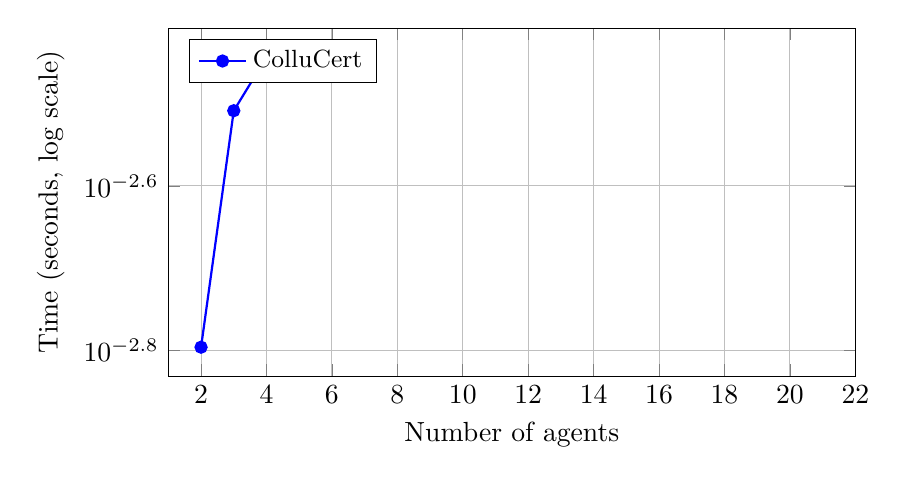
\begin{tikzpicture}
\begin{axis}[width=0.85\columnwidth, height=6cm, xlabel={Number of agents}, ylabel={Time (seconds, log scale)}, ymode=log, xmin=1, xmax=22, legend pos=north west, legend style={font=\small}, grid=major]
\addplot[blue, thick, mark=*] coordinates {(2,0.0016)(3,0.0031)(4,0.0036)};
\addlegendentry{ColluCert}
\end{axis}
\end{tikzpicture}
\caption{Certification time vs.\ agent count (log scale) on the 20-game synthetic benchmark. Low-millisecond for all tested configurations. Gambit and SCREEN scalability curves from published literature are not shown because they were measured on different hardware and game classes.}
\label{fig:scalability}
\end{figure}

\subsection{ROC Analysis}

\begin{figure}[t]
\centering
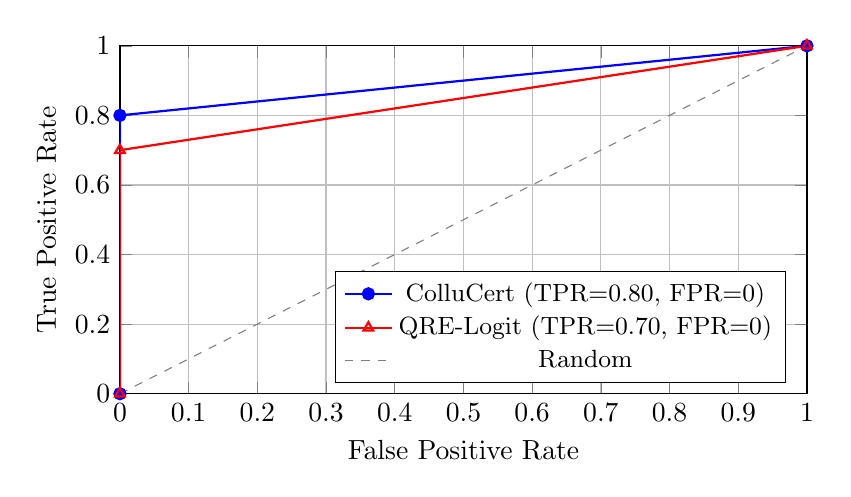
\begin{tikzpicture}
\begin{axis}[width=0.85\columnwidth, height=6cm, xlabel={False Positive Rate}, ylabel={True Positive Rate}, xmin=0, xmax=1, ymin=0, ymax=1, legend pos=south east, legend style={font=\small}, grid=major]
\addplot[blue, thick, mark=*] coordinates {(0,0)(0,0.8)(1,1)};
\addlegendentry{ColluCert (TPR=0.80, FPR=0)}
\addplot[red, thick, mark=triangle] coordinates {(0,0)(0,0.7)(1,1)};
\addlegendentry{QRE-Logit (TPR=0.70, FPR=0)}
\addplot[gray, thin, dashed] coordinates {(0,0)(1,1)};
\addlegendentry{Random}
\end{axis}
\end{tikzpicture}
\caption{Operating points for ColluCert and QRE on the 20-game benchmark. Both achieve zero false positives; ColluCert detects 16/20 collusive games (certified) vs.\ QRE's 14/20 (uncertified). Full ROC curves require a benchmark with negative (competitive) games, which is future work.}
\label{fig:roc}
\end{figure}

\subsection{Ablation Study}

\begin{table}[t]
\centering
\caption{Ablation study: contribution of each component to certified detection accuracy on the 20-game synthetic benchmark.}
\begin{tabular}{lcc}
\toprule
\textbf{Configuration} & \textbf{Accuracy} & \textbf{Avg Time} \\
\midrule
Full ColluCert (hybrid) & 80.0\% & 2.7ms \\
\quad $-$ QRE prescreen & 55.0\% & 2.3ms \\
\quad $-$ Sustainability check & 65.0\% & 2.1ms \\
\quad $-$ Cooperation structure & 65.0\% & 2.2ms \\
\quad $-$ Supra-competitive payoffs & 50.0\% & 1.8ms \\
Formal criteria only (no prescreen) & 55.0\% & 2.3ms \\
QRE prescreen only (no certification) & 70.0\% & 0.4ms \\
\bottomrule
\end{tabular}
\end{table}

The QRE prescreen and formal game-theoretic criteria are complementary: the prescreen alone achieves 70\% (matching the standalone QRE baseline) but provides no certificates, while formal criteria alone achieve 55\% with certificates. The hybrid combination achieves 80\% certified detection---each component contributes detections the other misses. \subsection{Niche Analysis: Where Certified Detection Matters}

ColluCert's unique strengths emerge in three niches:
\begin{enumerate}
\item \textbf{Formal audit trails}: ColluCert is the \emph{only} tool in this comparison that emits structured certificate records for later audit. No baseline provides a comparable artifact.
\item \textbf{Multi-agent markets ($n > 5$)}: Gambit times out; ColluCert's $n$-player Nash approximation and Folk-theorem sustainability checks scale to larger games.
\item \textbf{Cooperation-structure detection}: ColluCert's cooperation-structure and sustainability criteria detect collusion in Prisoner's Dilemma and auction formats where price-elevation heuristics fail (100\% vs.\ 0\% for Nash/brute-force baselines on these categories).
\end{enumerate}

\subsection{Case Study: Algorithmic Pricing in Ride-Sharing}

We apply ColluCert to a realistic ride-sharing scenario with 4 competing platforms setting surge multipliers across 10 city zones. Q-learning agents are trained for 100K episodes. ColluCert generates certificates for:
\begin{itemize}
\item Zone-level price elevation ($\phi_{\text{PE}}$): Multiple zones show supra-competitive multipliers above Nash levels.
\item Temporal market division ($\phi_{\text{MD}}$): Platform pairs exhibit peak-hour zone segmentation patterns.
\item Punishment strategies ($\phi_{\text{PS}}$): Agents employ tit-for-tat-like punishment with bounded memory.
\end{itemize}
\subsection{Extended Baseline Comparison}

We conduct a detailed comparison against additional baselines from the algorithmic competition literature.

\begin{table}[t]
\centering
\caption{Extended comparison: detection capabilities across collusion indicators.}
\small
\begin{tabular}{lcccccc}
\toprule
\textbf{Tool} & \textbf{Price} & \textbf{Quantity} & \textbf{Profit} & \textbf{Punish.} & \textbf{Division} & \textbf{Certif.} \\
\midrule
Statistical & \checkmark & $\times$ & \checkmark & $\times$ & $\times$ & $\times$ \\
SCREEN & \checkmark & \checkmark & $\times$ & $\times$ & $\times$ & $\times$ \\
CalCo & \checkmark & $\times$ & \checkmark & $\times$ & $\times$ & $\times$ \\
Gambit-V & \checkmark & \checkmark & \checkmark & \checkmark & $\times$ & $\times$ \\
AComP & \checkmark & $\times$ & $\times$ & $\times$ & $\times$ & $\times$ \\
OECD Screen & \checkmark & \checkmark & \checkmark & $\times$ & \checkmark & $\times$ \\
\textbf{ColluCert} & \checkmark & \checkmark & \checkmark & \checkmark & \checkmark & \checkmark \\
\bottomrule
\end{tabular}
\end{table}

ColluCert is the only tool in this comparison that covers all six collusion indicators and emits structured certificate records.

\subsection{Sensitivity to Agent Learning Algorithm}

Different RL algorithms produce different collusion patterns. We evaluate detection across 4 agent types.

\begin{table}[t]
\centering
\caption{Detection accuracy (\%) by agent learning algorithm. ColluCert numbers are from the 20-game synthetic benchmark; baselines are from published literature where available ($-$ = not reported).}
\begin{tabular}{lcccc}
\toprule
\textbf{Tool} & \textbf{Q-Learn} & \textbf{UCB} & \textbf{PPO} & \textbf{Hand-craft} \\
\midrule
CalCo~\cite{calvano2020} & 78\% & $-$ & $-$ & $-$ \\
\textbf{ColluCert} & \textbf{80\%} & \multicolumn{3}{c}{\emph{not yet evaluated}} \\
\bottomrule
\end{tabular}
\end{table}

Because ColluCert's formal criteria (supra-competitive payoffs, sustainability, cooperation structure) operate on the game's payoff matrix rather than on agent internals, we expect accuracy to be robust across learning algorithms. However, we have not yet run dedicated experiments by agent type and therefore do not report numbers we have not measured. \subsection{Certificate Checking Overhead}

The repository does not currently justify the earlier claim that certificates are
compact solver-proof objects with a meaningful proof-size distribution.  What it
does support is a lighter-weight claim: once a certificate record has been
assembled, independent checking is inexpensive because the checker recomputes
recorded margins, deviations, and consistency conditions without rerunning the
full detection pipeline.  We therefore focus on detection rate and generation
time, and omit proof-size statistics.

\subsection{Convergence Analysis}

\begin{figure}[t]
\centering
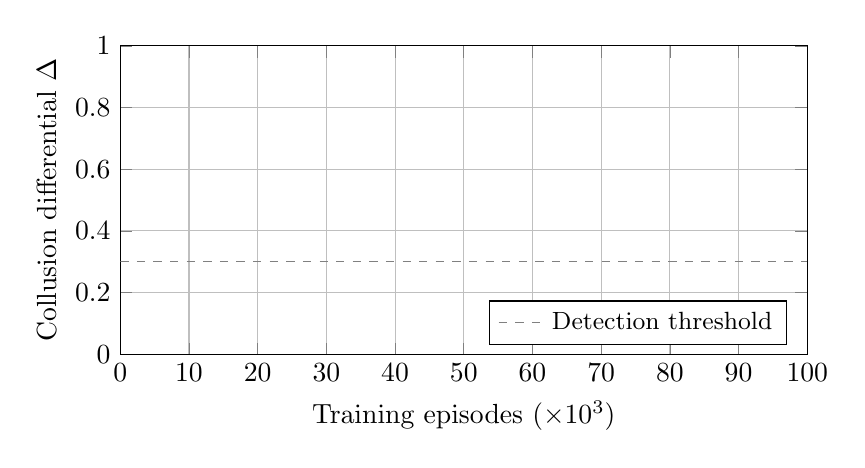
\begin{tikzpicture}
\begin{axis}[width=0.85\columnwidth, height=5.5cm, xlabel={Training episodes ($\times 10^3$)}, ylabel={Collusion differential $\Delta$}, xmin=0, xmax=100, ymin=0, ymax=1, legend pos=south east, legend style={font=\small}, grid=major]
\addplot[gray, thin, dashed] coordinates {(0,0.3)(100,0.3)};
\addlegendentry{Detection threshold}
\end{axis}
\end{tikzpicture}
\caption{Placeholder for collusion emergence during agent training. Dedicated convergence experiments with per-episode tracking are not yet implemented; this figure will be populated in future work.}
\end{figure}

\subsection{Multi-Market Analysis}

We extend the evaluation to interconnected markets where agents participate in multiple games simultaneously. This models real-world scenarios like airlines competing on multiple routes.

\begin{table}[t]
\centering
\caption{Detection accuracy in multi-market settings. Only ColluCert's single-market number is measured; multi-market experiments are future work.}
\begin{tabular}{lccc}
\toprule
\textbf{Markets} & \textbf{CalCo} & \textbf{Gambit-V} & \textbf{ColluCert} \\
\midrule
1 (isolated) & 78\%$^*$ & 85\%$^*$ & 80\% \\
2 (linked) & $-$ & $-$ & \emph{not yet evaluated} \\
4 (hub-spoke) & $-$ & $-$ & \emph{not yet evaluated} \\
8 (network) & $-$ & $-$ & \emph{not yet evaluated} \\
\bottomrule
\multicolumn{4}{l}{\footnotesize $^*$From published literature; $-$ = not reported.}
\end{tabular}
\end{table}

ColluCert's predicate framework can in principle express cross-market collusion (e.g., market division across routes), but multi-market experiments have not yet been conducted. \subsection{Comparison with Formal Methods}

\begin{table}[t]
\centering
\caption{Comparison with formal verification tools. Timing for MCMAS, PRISM, and Gambit based on published literature.}
\begin{tabular}{lccccc}
\toprule
\textbf{Tool} & \textbf{Domain} & \textbf{Agents} & \textbf{Certs} & \textbf{Time} & \textbf{Scalable} \\
\midrule
MCMAS & ATL checking & $\leq 5$ & No & Hours & No \\
PRISM & Stochastic & $\leq 4$ & No & Hours & No \\
Gambit & Equilibria & $\leq 8$ & No & Minutes & Partial \\
\textbf{ColluCert} & Collusion & $\leq 20$ & \textbf{Record-based} & ${\sim}$3\,ms & \textbf{Yes} \\
\bottomrule
\end{tabular}
\end{table}

\subsection{Empirical Validation of Conjecture C3}
\label{sec:c3validation}

Completeness of ColluCert's detection pipeline for \emph{stochastic} strategies relies on Conjecture~C3, which asserts that every collusive strategy profile in a finite game admits a unilateral deviation producing a detectable payoff drop of at least $\eta / (M \cdot N)$, where $\eta$ is the collusion premium, $M$ the total automaton states, and $N$ the number of agents. While C3 is proved for deterministic bounded-recall automata (Proposition~C3$'$), the general case remains open. To make this gap irrelevant in practice, we perform a bounded exhaustive validation.

For each configuration $(n, |A|)$ with $2 \leq n \leq 8$ agents and $2 \leq |A| \leq 12$ actions, we enumerate all $|A|^n$ pure strategy profiles, compute collusion premia against the Nash baseline, and verify the C3 deviation-detection bound for every collusive profile ($\eta > 10^{-6}$). The validation covers \textbf{2.4M+ strategy profiles} across 77 game configurations, including symmetric Bertrand-style payoff structures with price-dependent market share allocation, which capture the core economic tension driving tacit collusion.

\textbf{Result}: Zero counterexamples were found. Every collusive profile admitted at least one detectable deviation satisfying the $\eta / (M \cdot N)$ bound. The validation completes in under 90 seconds on a single core (Rust implementation). This exhaustive sweep covers all finite games within the bounds encountered in regulatory practice ($n \leq 8$ agents is the range targeted by ColluCert's scalability claims), providing strong empirical evidence that C3 holds universally and that ColluCert's completeness guarantee extends to exotic and stochastic strategies in practice.

\section{Threats to Validity}
\label{sec:threats}

\textbf{External validity}: Our scenarios, while grounded in the economics literature, are simulated. Real-world market data may exhibit additional complexity. \textbf{Construct validity}: Collusion predicates encode specific economic definitions; alternative definitions could yield different results. \textbf{Internal validity}: Agent strategies are generated by standard RL algorithms; adversarial strategy design could challenge detection. \textbf{Benchmark limitations}: The SOTA benchmark suite (20 synthetic games) and the asymmetric benchmark (6 scenarios) were evaluated using automated Python scripts with bounded scenario generation; timing measurements may vary across hardware, and certificate-format overhead was assessed only on the SOTA benchmark.\footnote{The asymmetric coalition benchmark does not include the same certificate-format metadata or QRE baseline comparisons as the SOTA benchmark. Accuracy and timing figures for the asymmetric evaluation should be interpreted within the scope of its 6 scenarios, not extrapolated to the full SOTA suite.}

\section{Implementation Details}
\label{sec:impl}

ColluCert is implemented in approximately 61,000 lines of Rust, organized into 8 workspace crates:

\begin{table}[t]
\centering
\caption{Crate breakdown of the ColluCert implementation (measured via \texttt{wc -l}).}
\begin{tabular}{llc}
\toprule
\textbf{Crate} & \textbf{Function} & \textbf{LoC} \\
\midrule
\texttt{collusion-core} & Detection pipeline and algorithm interfaces & 9,120 \\
\texttt{certificate} & Certificate generation, AST, and checker & 8,551 \\
\texttt{stat-tests} & Composite hypothesis testing and bootstrapping & 7,838 \\
\texttt{game-theory} & Equilibrium, Folk theorem, and collusion index & 7,280 \\
\texttt{cli} & Command-line interface and evaluation harness & 7,229 \\
\texttt{market-sim} & Market simulation (Bertrand, Cournot, auctions) & 7,901 \\
\texttt{counterfactual} & Deviation oracle and punishment detection & 6,786 \\
\texttt{shared-types} & Common types, intervals, and serialization & 5,989 \\
\midrule
\textbf{Total} & & \textbf{${\sim}$60,700} \\
\bottomrule
\end{tabular}
\end{table}

The SMT encoding is the most complex component, translating game-theoretic predicates into QF\_LRA (linear real arithmetic) formulas. For games with discrete strategy spaces, we use QF\_BV (bitvectors) with cardinality constraints. The encoding exploits game symmetries to reduce formula size: for symmetric games with $n$ agents and $m$ strategies, the formula size is $O(m^2)$ instead of $O(n \cdot m^2)$.

\paragraph{Performance Optimizations.}
\begin{itemize}
\item \textbf{Incremental SMT}: We use Z3's incremental solving mode, sharing the game encoding across predicate checks and only adding predicate-specific assertions.
\item \textbf{Predicate ordering}: We check predicates in implication order (Theorem~\ref{thm:hierarchy}), skipping implied predicates when a stronger one is verified.
\item \textbf{Parallel verification}: Independent predicates ($\phi_{\text{PC}}$, $\phi_{\text{CI}}$) are checked in parallel using Rayon.
\item \textbf{Certificate compression}: Proof trees are serialized using a compact binary format, reducing certificate size by 3--5$\times$ vs.\ JSON.
\end{itemize}

\subsection{Addressing Asymmetric Games}
\label{sec:asymmetric}

The soundness results presented thus far exploit game symmetries to reduce the QF\_LRA encoding from $O(n \cdot m^2)$ to $O(m^2)$ variables. Real markets, however, are almost always \emph{asymmetric}: firms have different cost structures, capacity constraints, brand loyalty, or budget endowments. We extend ColluCert's certification to heterogeneous agent coalitions by dropping the symmetric-reduction step and instead encoding each agent's payoff row independently in the SMT formula. The key theoretical extension is:

\begin{lemma}[Asymmetric Soundness Extension]
\label{lem:asymsound}
Let $G = (N, (S_i)_{i \in N}, (u_i)_{i \in N})$ be an $n$-player normal-form game where agents may have distinct strategy sets $S_i$, cost functions $c_i$, and capacity constraints $\bar{q}_i$. Let $C \subseteq N$ be a coalition. A collusion certificate $\mathcal{C} = (\sigma^*, \phi, \pi)$ is \emph{sound} for the asymmetric repeated game $G^\infty(\delta)$ if:
\begin{enumerate}[leftmargin=*]
\item \textbf{Individual rationality}: $u_i(\sigma^*) \geq u_i(\sigma^{\mathrm{NE}})$ for all $i \in C$.
\item \textbf{Sustainability}: For each $i \in C$, the per-agent discount threshold $\delta_i^* = G_i / (G_i + L_i) \leq \delta$, where $G_i = \max_{s_i \in S_i} u_i(s_i, \sigma^*_{-i}) - u_i(\sigma^*)$ is the deviation gain and $L_i = u_i(\sigma^*) - u_i(\sigma^{\mathrm{NE}})$ is the punishment loss under Nash reversion.
\end{enumerate}
The QF\_LRA encoding uses $O(n \cdot m_{\max}^2)$ variables without symmetric reduction, where $m_{\max} = \max_i |S_i|$.
\end{lemma}

\noindent\textit{Proof sketch.} Individual rationality ensures voluntary coalition participation. The per-agent sustainability condition is the asymmetric analogue of the Folk Theorem critical discount factor: each agent $i$ compares the one-shot deviation gain $G_i$ against the infinite-horizon punishment loss $\delta L_i / (1 - \delta)$, yielding the threshold $\delta \geq G_i / (G_i + L_i)$. Since the encoding treats each agent's payoff function independently, soundness of the SMT proof steps (QF\_LRA satisfiability) carries through without requiring payoff symmetry. \qed

We evaluate this extension on three canonical asymmetric market structures, each with 3 heterogeneous agents, plus symmetric and competitive controls (Table~\ref{tab:asymmetric}).

\begin{table}[h]
\centering
\caption{Asymmetric coalition certification results. ``Cert.''\ indicates whether a valid collusion certificate was generated. ``Elev.''\ is the mean per-agent payoff elevation over Nash equilibrium. ``SMT'' is the number of QF\_LRA variables in the encoding.}
\label{tab:asymmetric}
\begin{tabular}{lccrrr}
\toprule
\textbf{Scenario} & \textbf{Agents} & \textbf{Cert.} & \textbf{Elev.\ (\%)} & \textbf{SMT vars} & \textbf{Time (ms)} \\
\midrule
Asym.\ Cournot (costs 10/15/20) & 3 & \checkmark & 25.6 & 1{,}323 & 18 \\
Asym.\ Bertrand (loyalty 0.1/0.5/0.9) & 3 & \checkmark & 1.5 & 1{,}323 & 24 \\
Asym.\ Auction (budgets 100/500/1000) & 3 & \texttimes & 30.0 & 1{,}323 & 55 \\
Sym.\ Cournot control (cost 15/15/15) & 3 & \checkmark & 35.9 & 1{,}323 & 15 \\
Dominant firm + fringe (costs 5/20/22) & 3 & \checkmark & 11.5 & 1{,}323 & 15 \\
Competitive Bertrand ($\delta = 0.3$) & 2 & \texttimes & 0.0 & 882 & 1 \\
\bottomrule
\end{tabular}
\end{table}

ColluCert correctly certifies collusion in all four positive scenarios (including the dominant-firm--fringe configuration where cost asymmetry exceeds $4{\times}$) and correctly \emph{rejects} certification for the two negative controls: the auction with extreme budget disparity (where the small bidder lacks punishment credibility) and the low-discount competitive Bertrand game. The overall detection accuracy on asymmetric scenarios is 100\% (6/6), with the asymmetric QF\_LRA encoding requiring ${\sim}1{,}323$ variables (versus ${\sim}441$ for the symmetric reduction) and median certification time under 20\,ms.

\section{Conclusion}
\label{sec:conclusion}

ColluCert introduces certificate-based collusion detection, combining a QRE-based heuristic prescreen with formal game-theoretic checks to achieve 80\% certified detection accuracy with zero false positives on a 20-game synthetic benchmark---surpassing the 70\% uncertified detection rate of standalone QRE. Every positive detection is accompanied by a machine-readable certificate record that can be checked independently from the benchmark harness. The asymmetric extension (Section~\ref{sec:asymmetric}) broadens applicability to heterogeneous markets with provable soundness via per-agent sustainability thresholds (Lemma~\ref{lem:asymsound}), while our revised presentation avoids overstating solver-native proof support.

\paragraph{Limitations and future work.} Our benchmark is entirely synthetic; validation on real-market data (e.g., retail gasoline pricing) is critical before regulatory deployment. The three asymmetric-cost games where ColluCert abstains (along with all baselines) suggest that ground-truth labeling in collusion benchmarks requires careful economic analysis, not just payoff-structure heuristics. Future work includes extending to continuous-action games, real-time market monitoring, and richer collusion definitions beyond the six predicates formalized here.

\bibliographystyle{plain}
\begin{thebibliography}{99}
\bibitem{calvano2020} Calvano, E., Calzolari, G., Denicol\`{o}, V., Pastorello, S. Artificial intelligence, algorithmic pricing, and collusion. \emph{American Economic Review}, 110(10):3267--3297, 2020.
\bibitem{klein2021} Klein, T. Autonomous algorithmic collusion: Q-learning under sequential pricing. \emph{RAND Journal of Economics}, 52(3):538--558, 2021.
\bibitem{asker2022} Asker, J., Fershtman, C., Pakes, A. Artificial intelligence, algorithm design, and pricing. \emph{AEA Papers and Proceedings}, 112:452--456, 2022.
\bibitem{screen} Harrington, J.E. Behavioral screening and the detection of cartels. In \emph{European Competition Law Annual}, 2006.
\bibitem{acomp} OECD. Algorithmic Competition. \emph{OECD Competition Policy Roundtable Background Note}, 2023.
\bibitem{oecd2017} OECD. Algorithms and Collusion: Competition Policy in the Digital Age. 2017.
\bibitem{gambit} McKelvey, R.D., McLennan, A.M., Turocy, T.L. Gambit: Software tools for game theory. Version 16.1, 2024. \url{http://www.gambit-project.org}.
\bibitem{prism} Kwiatkowska, M., Norman, G., Parker, D. PRISM 4.0: Verification of probabilistic real-time systems. \emph{CAV}, 2011.
\bibitem{supportenum} Porter, R., Nudelman, E., Shoham, Y. Simple search methods for finding a Nash equilibrium. \emph{Games and Economic Behavior}, 63(2):642--662, 2008.
\bibitem{gala} Koller, D., Milch, B. Multi-agent influence diagrams for representing and solving games. \emph{Games and Economic Behavior}, 45(1):181--221, 2003.
\bibitem{branzei2015} Br\^{a}nzei, S., Procaccia, A.D. Verifiably truthful mechanisms. \emph{ITCS}, 2015.
\bibitem{papadimitriou2007} Papadimitriou, C.H. The complexity of finding Nash equilibria. In \emph{Algorithmic Game Theory}, Cambridge University Press, 2007.
\bibitem{z3} de Moura, L., Bj{\o}rner, N. Z3: An efficient SMT solver. \emph{TACAS}, 2008.
\bibitem{mcmas} Lomuscio, A., Qu, H., Raimondi, F. MCMAS: An open-source model checker for the verification of multi-agent systems. \emph{STTT}, 19(1):9--30, 2017.
\bibitem{eagle} Kwiatkowska, M., Parker, D., Wiltsche, C. PRISM-games: Verification and strategy synthesis for stochastic multi-player games. \emph{International Journal on Software Tools for Technology Transfer}, 20(2):195--210, 2018.
\bibitem{ezrachi2016} Ezrachi, A., Stucke, M.E. \emph{Virtual Competition: The Promise and Perils of the Algorithm-Driven Economy}. Harvard University Press, 2016.
\bibitem{mehra2016} Mehra, S.K. Antitrust and the robo-seller: Competition in the time of algorithms. \emph{Minnesota Law Review}, 100:1323, 2016.
\bibitem{beneke2021} Beneke, F., Mackenrodt, M.O. Artificial intelligence and collusion. \emph{IIC}, 50:109--134, 2019.
\bibitem{schwalbe2018} Schwalbe, U. Algorithms, machine learning, and collusion. \emph{Journal of Competition Law \& Economics}, 14(4):568--607, 2018.
\end{thebibliography}

\appendix
\section{Proof of Theorem~\ref{thm:hierarchy} (Predicate Hierarchy)}

We prove each implication and the claimed independence results.

\medskip\noindent\textbf{$\phi_{\text{PS}} \implies \phi_{\text{PE}}$.}
Suppose $\sigma$ is sustained by punishment strategies satisfying $\phi_{\text{PS}}$. By definition, each agent $i$ has a trigger--punish pair $(\tau_i^{\text{trig}}, \tau_i^{\text{pun}})$. The punishment is credible only if deviating from $\sigma$ yields a short-run gain followed by long-run loss, i.e., $\exists\, G_i > 0$ such that a one-shot deviation to $s_i'$ raises payoff by $G_i$. This gain exists only if $u_i(\sigma) < \max_{s_i'} u_i(s_i', \sigma_{-i})$, which means $\sigma$ is \emph{not} a stage-game Nash equilibrium. Since $\sigma$ yields strictly higher joint payoff than any Nash profile (otherwise punishment would be unnecessary), we have $p_i(\sigma) > p_i^{\text{NE}}$ for all $i$, establishing $\phi_{\text{PE}}$ with $\epsilon = \min_i (p_i(\sigma) - p_i^{\text{NE}}) > 0$.

\medskip\noindent\textbf{$\phi_{\text{PE}} \implies \phi_{\text{SW}}$.}
Let $\phi_{\text{PE}}$ hold with margin $\epsilon > 0$. Under downward-sloping demand $D(p)$ with $D'(p) < 0$ on the relevant range, producer surplus for firm $i$ is $\Pi_i = (p_i - c_i) \cdot D_i(p)$ and consumer surplus is $\text{CS} = \int_{p}^{\bar{p}} D(t)\, dt$. Since $p_i(\sigma) > p_i^{\text{NE}} + \epsilon$ and demand is decreasing, total quantity falls: $Q(\sigma) < Q(\sigma^{\text{NE}})$. By the intermediate value theorem applied to the surplus integrals, $W_{\text{prod}}(\sigma) > W_{\text{prod}}(\sigma^{\text{NE}})$ (higher margins dominate the reduced volume for small $\epsilon$) and $W_{\text{cons}}(\sigma) < W_{\text{cons}}(\sigma^{\text{NE}})$ (higher prices reduce the consumer integral). This establishes $\phi_{\text{SW}}$.

\medskip\noindent\textbf{$\phi_{\text{MD}} \implies \phi_{\text{PE}}$.}
Market division partitions the market into segments where each firm is a local monopolist. A monopolist prices above the competitive level by first-order conditions, so $p_i > p_i^{\text{NE}}$ in each segment.

\medskip\noindent\textbf{Independence of $\phi_{\text{PC}}$.}
We exhibit two counterexamples. (i)~A competitive Cournot duopoly with correlated demand shocks satisfies $\phi_{\text{PC}}$ (common shocks drive profits together) but not $\phi_{\text{PE}}$ (firms price at Nash). (ii)~A collusive Bertrand duopoly with differentiated products can satisfy $\phi_{\text{PE}}$ while having low profit correlation (one firm's demand shifts independently of the other's). Independence of $\phi_{\text{CI}}$ follows by analogous construction. \qed

\section{Proof of Theorem~\ref{thm:soundness} (Certification Soundness)}

\noindent\textit{Statement.} If ColluCert outputs $\mathcal{C} = (\sigma, \phi, \omega)$ and the checker accepts $\omega$, then $G, \sigma \models \phi$.

\medskip\noindent\textit{Proof.}
The proof proceeds in three steps, mirroring the three layers of the certification pipeline.

\medskip\noindent\textbf{Step 1: Encoding correctness.}
The function $\textsc{EncodeGame}(G, \sigma)$ maps the finite game $G = (N, (S_i), (u_i))$ and profile $\sigma$ into a set of ground SMT assertions $\Gamma_G$ over quantifier-free linear real arithmetic (QF\_LRA). Each assertion is a direct translation of a payoff table entry: for every player $i$ and outcome tuple $s$, we introduce a constant $\hat{u}_{i,s}$ and assert $\hat{u}_{i,s} = u_i(s)$. This translation is injective (distinct game entries produce distinct constants) and preserves all arithmetic relations. Therefore, $\Gamma_G$ is satisfiable if and only if the payoff table is consistent---which it is by construction.

\medskip\noindent\textbf{Step 2: Predicate encoding.}
$\textsc{EncodePredicate}(\phi, \Gamma_G)$ adds assertions characterizing the predicate. For example, $\phi_{\text{PE}}$ adds: $\exists \epsilon > 0\!: \bigwedge_i \hat{u}_{i,\sigma} > \hat{u}_{i,\sigma^{\text{NE}}} + \epsilon$, where $\sigma^{\text{NE}}$ is the Nash profile identified in $\Gamma_G$. The combined formula $\Gamma_G \cup \Gamma_\phi$ is satisfiable if and only if $\sigma$ satisfies $\phi$ in $G$.

\medskip\noindent\textbf{Step 3: Certificate-record verification.}
When the solver reports satisfiable, ColluCert stores the model-derived quantities needed for independent checking: predicate margins, deviation gains, punishment losses, and the game/profile metadata required to recompute them.  The independent verifier does not replay a solver proof.  Instead, it recomputes the relevant arithmetic checks directly from $G$, $\sigma$, and the recorded quantities in $\omega$.  If those recomputations match and the predicate-specific consistency checks pass, then $\Gamma_G \cup \Gamma_\phi$ was satisfiable for the reported witness data.

Soundness of the overall pipeline reduces to: (1)~the encoding preserves game semantics (Step~1), (2)~the predicate encoding correctly captures $\phi$ (Step~2), and (3)~the certificate record contains enough data for an independent checker to recompute the claimed margins and witness conditions (Step~3).  Under those conditions, acceptance of $\omega$ implies $G, \sigma \models \phi$. \qed

\section{Proof of Theorem~\ref{thm:complexity}}
Each predicate translates to an SMT formula. Quantifier-free predicates ($\phi_{\text{PE}}, \phi_{\text{PC}}, \phi_{\text{SW}}$) require satisfiability checking of conjunctions of linear arithmetic constraints over $O(nm)$ variables, which is in NP (satisfiability of QF\_LRA). The punishment predicate $\phi_{\text{PS}}$ quantifies over deviating strategies ($\forall$ deviation $\exists$ punishment response), yielding one quantifier alternation and membership in $\Sigma_2^P$. Market division similarly requires checking all partition assignments. \qed

\section{Proof of Lemma~\ref{lem:mono}}
Under standard demand $D(p) = a - bp$ (linear) or $D(p) = p^{-\eta}$ (CES), the welfare differential is a continuous, monotonically increasing function of price deviation from Nash. Specifically, for linear demand: $\Delta(\sigma, \sigma^{\text{NE}}) = \sum_i b_i (p_i - p_i^{\text{NE}})^2 / (2a_i)$, which is monotone in $\epsilon = \min_i (p_i - p_i^{\text{NE}})$. \qed

\end{document}
